\documentclass{article}
\usepackage[utf8]{inputenc}
\usepackage{amssymb}
\usepackage{graphicx}
\usepackage{setspace}
\usepackage{listings}
\usepackage{float}
\usepackage{xcolor}
\usepackage{amsmath}
\usepackage{pgfplots}
\usepackage{subcaption}
\usepackage{hyperref}

\title{\textbf{High Performance Computer Architectures Practical Course \\ - Exercise 6 -} \\[10mm]}
\author{Tutorium 1 \\[10mm] David Jordan (6260776) \\[1mm] Florian Rüffer (7454628) \\[1mm] Michael Samjatin (7485765) \\[10mm]}


\lstset{
    language=C++,
    basicstyle=\ttfamily,
    keywordstyle=\color{blue},
    stringstyle=\color{red},
    commentstyle=\color{green},
    numbers=left,
    numberstyle=\normalsize,
    breaklines=true,
    showstringspaces=false,
    frame=single,
    linewidth=1\linewidth,
    captionpos=b
}
\renewcommand{\lstlistingname}{File}% Listing -> Algorithm
\renewcommand{\lstlistlistingname}{List of \lstlistingname s}% List of Listings -> List of Algorithms

\begin{document}
\maketitle
\newpage
\section*{Section FittingDemoSimple\_0}
The 'fitFunction' function has the purpose to define the funtional form of the background model. This model will then be fitted to the histogram data. Root framework will attempt to find the best fit of the parameters so that the difference between the histogram data and the model is minimized.
In the 'FittingDemoSimple0' function we create the canvas to display the ROOT objects, we fill it with 1 000 000 random numbers we generate. 
We create a TF1, which represents the quadratic function defined earlier. The histogram is then fitted with the Fit method of the histogram. 
So the program has in effect created a histogram filled with random numbers from a triangular distribution, which is then fitted with a quadratic function. The graph it creates shows this fitted quadratic function overlaid over the histogram, in order to show how well the function fits the data.

Below we can see the output graphs:
\begin{figure}[H]
    \centering
    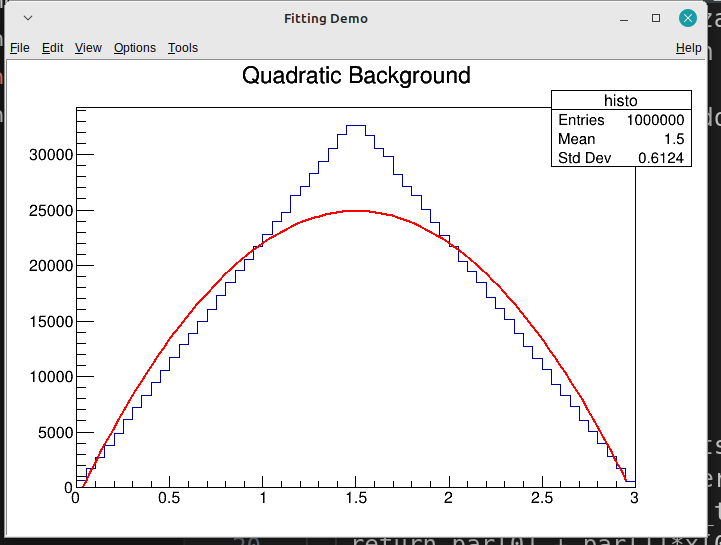
\includegraphics[scale=0.3]{graph.png} 
    \caption{Histogram}
    \label{fig:graph}
  \end{figure}

And the output metrics:

 \begin{figure}[H]
    \centering
    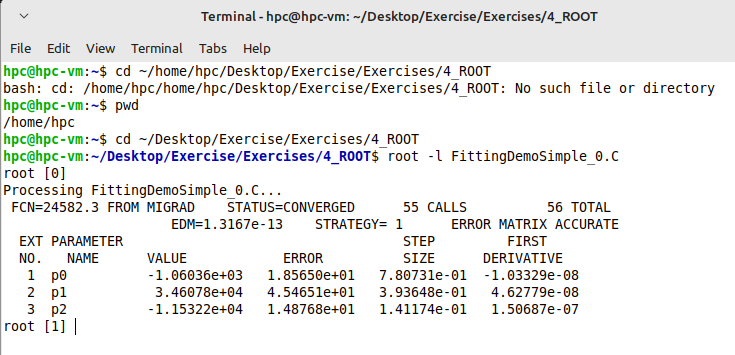
\includegraphics[scale=0.3]{metrics.png} 
    \caption{Histogram}
    \label{fig:graph}
    \end{figure}

\section*{Section 1}

First and foremost, we must decide which data should be
grouped and how it should be grouped in order to vectorize
the track fitting procedure.
To achieve maximum independence, M tracks can be handled simultaneously.
The procedure involves:

\section*{FittingDemo\_1}
To accomplish this task we need to adjust the polynomial order of our background function
to the order of three, four and six. We do this with the following code snippets: \\[3mm]

\begin{lstlisting}[caption=Order 3]
    Double_t background(Double_t *x, Double_t *par) {
   return par[0] + par[1]*x[0] + par[2]*x[0]*x[0] + par[3]*x[0]*x[0]*x[0];
}

\end{lstlisting}
\begin{lstlisting}[caption=Order 4]
    Double_t background(Double_t *x, Double_t *par) {
        return par[0] + par[1]*x[0] + par[2]*x[0]*x[0] + par[3]*x[0]*x[0]*x[0] + par[4]*x[0]*x[0]*x[0]*x[0];
     }
     
\end{lstlisting}
\begin{lstlisting}[caption=Order 6]
    Double_t background(Double_t *x, Double_t *par) {
        return par[0] + par[1]*x[0] + par[2]*x[0]*x[0] + par[3]*x[0]*x[0]*x[0] + par[4]*x[0]*x[0]*x[0]*x[0] + par[5]*x[0]*x[0]*x[0]*x[0]*x[0] + par[6]*x[0]*x[0]*x[0]*x[0]*x[0]*x[0];
     }
     

\end{lstlisting}

In the code snippets above the function 'background' takes two parameters x and the value par, which denotes
an array of parameters (six in total).

  
\end{document}